\documentclass[12pt,a4paper]{article}
\usepackage[utf8]{inputenc}
\usepackage[french]{babel}
\usepackage[T1]{fontenc}
\usepackage{amsmath}
\usepackage{amsfonts}
\usepackage{amssymb}
\usepackage{graphicx}
\usepackage[left=2cm,right=2cm,top=2cm,bottom=2cm]{geometry}
\author{KONDI Abdoul malik \\ NGANDEU NDJEUKAM Alhasan}
\title{Manuelle d'utilisation de l'application de gestion de la médiathèque}
\begin{document}
\maketitle
\tableofcontents
\newpage

\section{Préambule}
Ce manuel d'utilisation ci explique comment utilisé le site web de la médiathèque afin
de permettre aux personnels de la médiathèque de ce familiariser avec ce dernier.

\newpage
\section{Se connecter à l'application}
Pour se connecter à l'application, cliquer sur le bouton se connecter.\\
Une nouvelle page vient d'apparaître. Renseigner votre e mail et votre mot de passe 
puis cliquer sur le bouton \textbf{SE CONNECTER}. C'est tous maintenant vous êtes 
connecté.


\newpage
\section{Gestion des utilisateurs}
Le menu gestion des utilisateurs comme vous pouvez facilement le deviné est un menu qui
nous permet de gérer les abonnés, leurs abonnements et le personnel (tous ce qui se
connecterons à l'application). Pour accéder à ce menu, vous devez cliquer sur le bouton sur le
quelle trois (3) traits on été marqué il se trouve à gauche de l'écran dans une barre
vertical. \\

\begin{center}
\begin{tabular}{|p{17cm}|}
\hline 
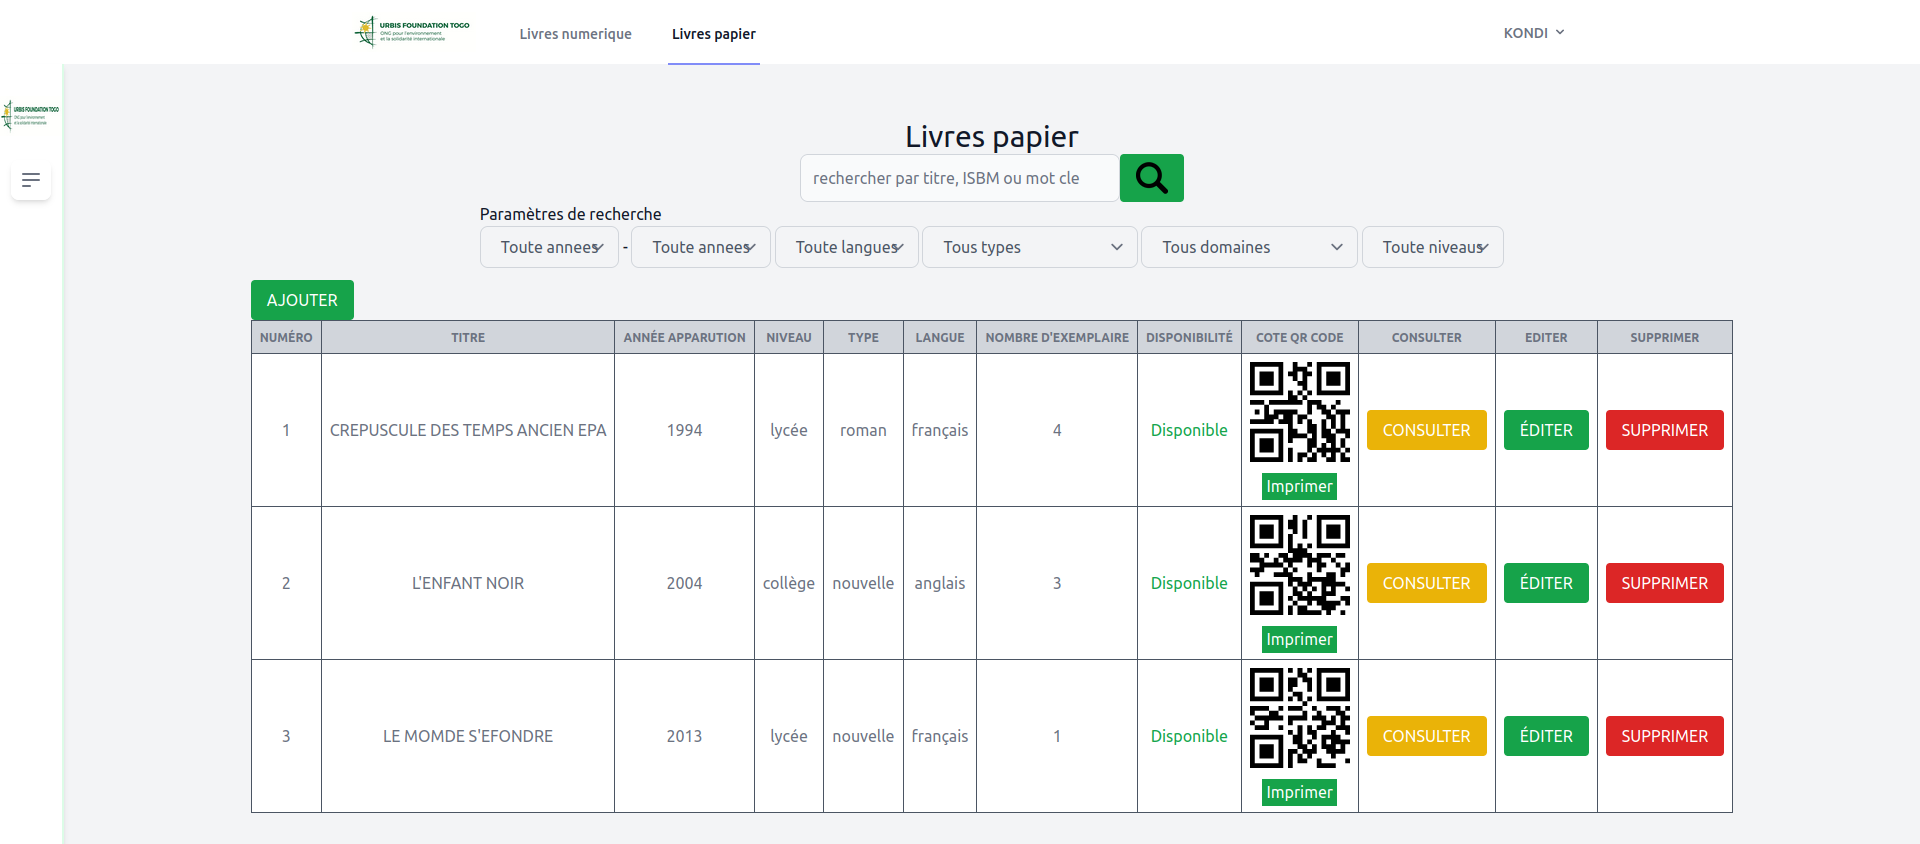
\includegraphics[width=\textwidth]{img/sidebar.png} \\ 
\hline 
\end{tabular} 
\end{center}

Une fois que vous avez cliquer sur ce bouton, vous remarquerez qu'un quart (1/4) de page 
sortira de la gauche de l'écran. Rendez vous maintenant au menu \textbf{Gestion des
utilisateurs} écrit en jaune. Vous y verrez trois sous menus :
\begin{itemize}
\item[•] Abonnés
\item[•] Abonnements
\item[•] Personnels
\end{itemize}

\begin{center}
\begin{tabular}{|p{17cm}|}
\hline 
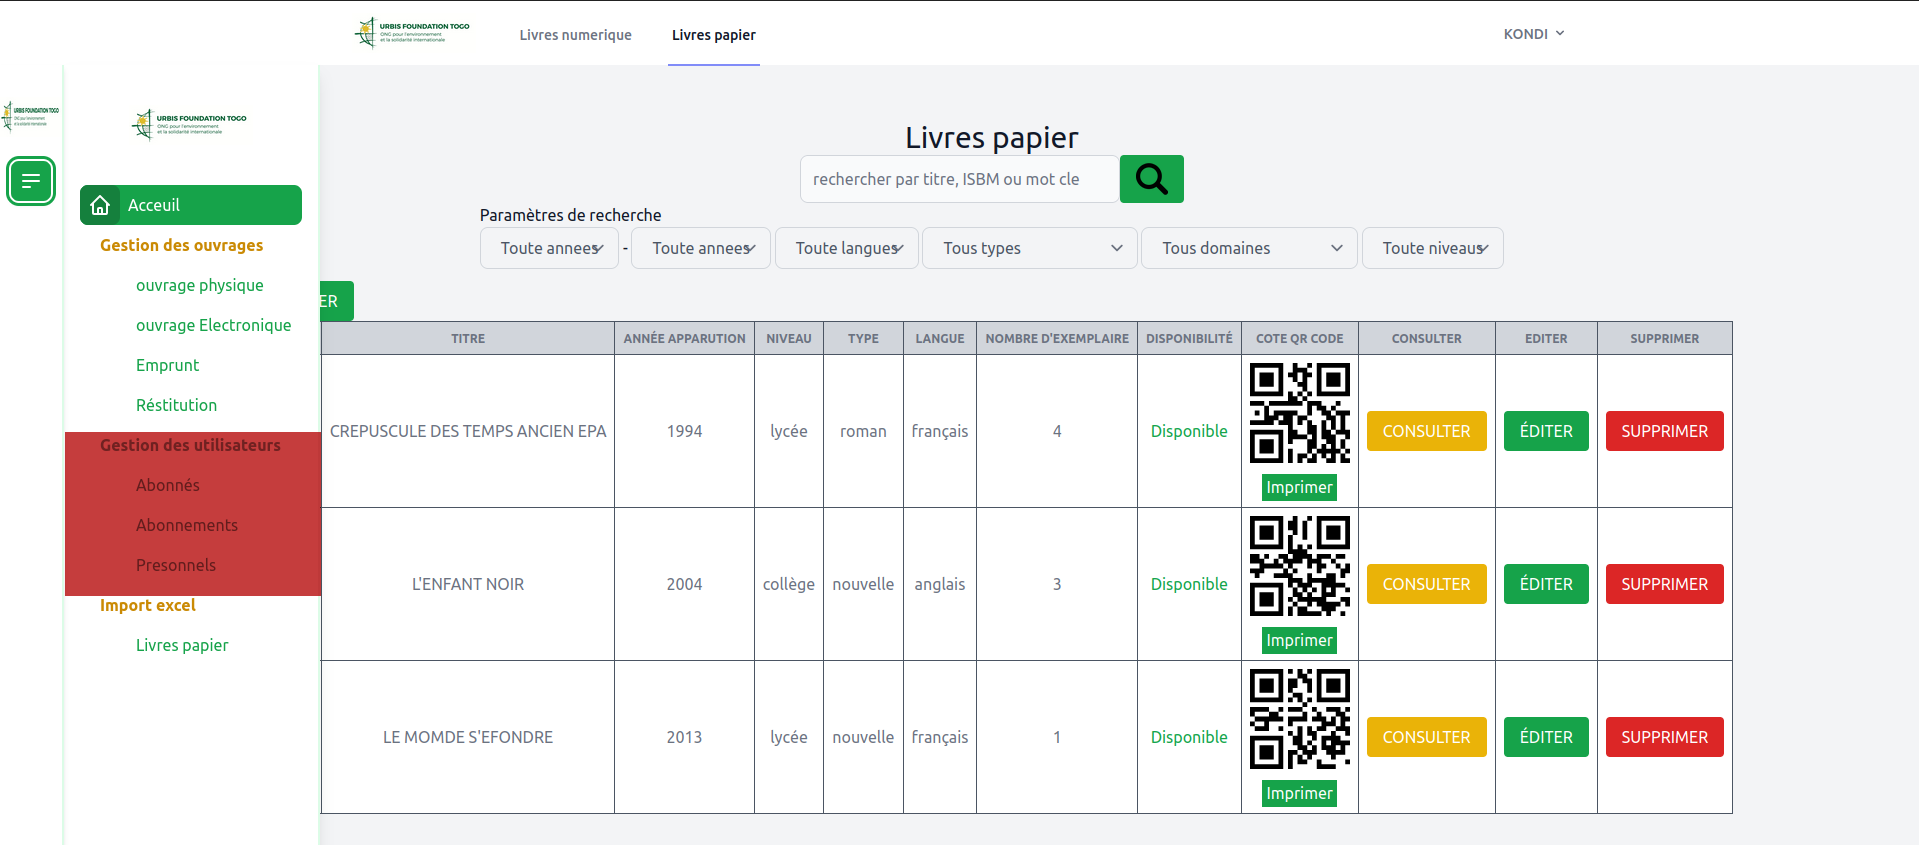
\includegraphics[width=\textwidth]{img/gestion_utilisateurs2.png} \\ 
\hline 
\end{tabular} 
\end{center}

\subsubsection{Sous menu \textbf{Abonnés}}
Cliquer sur \textbf{Abonnés} vous verrez cette page s'afficher.\\
\begin{center}
\begin{tabular}{|p{17cm}|}
\hline 
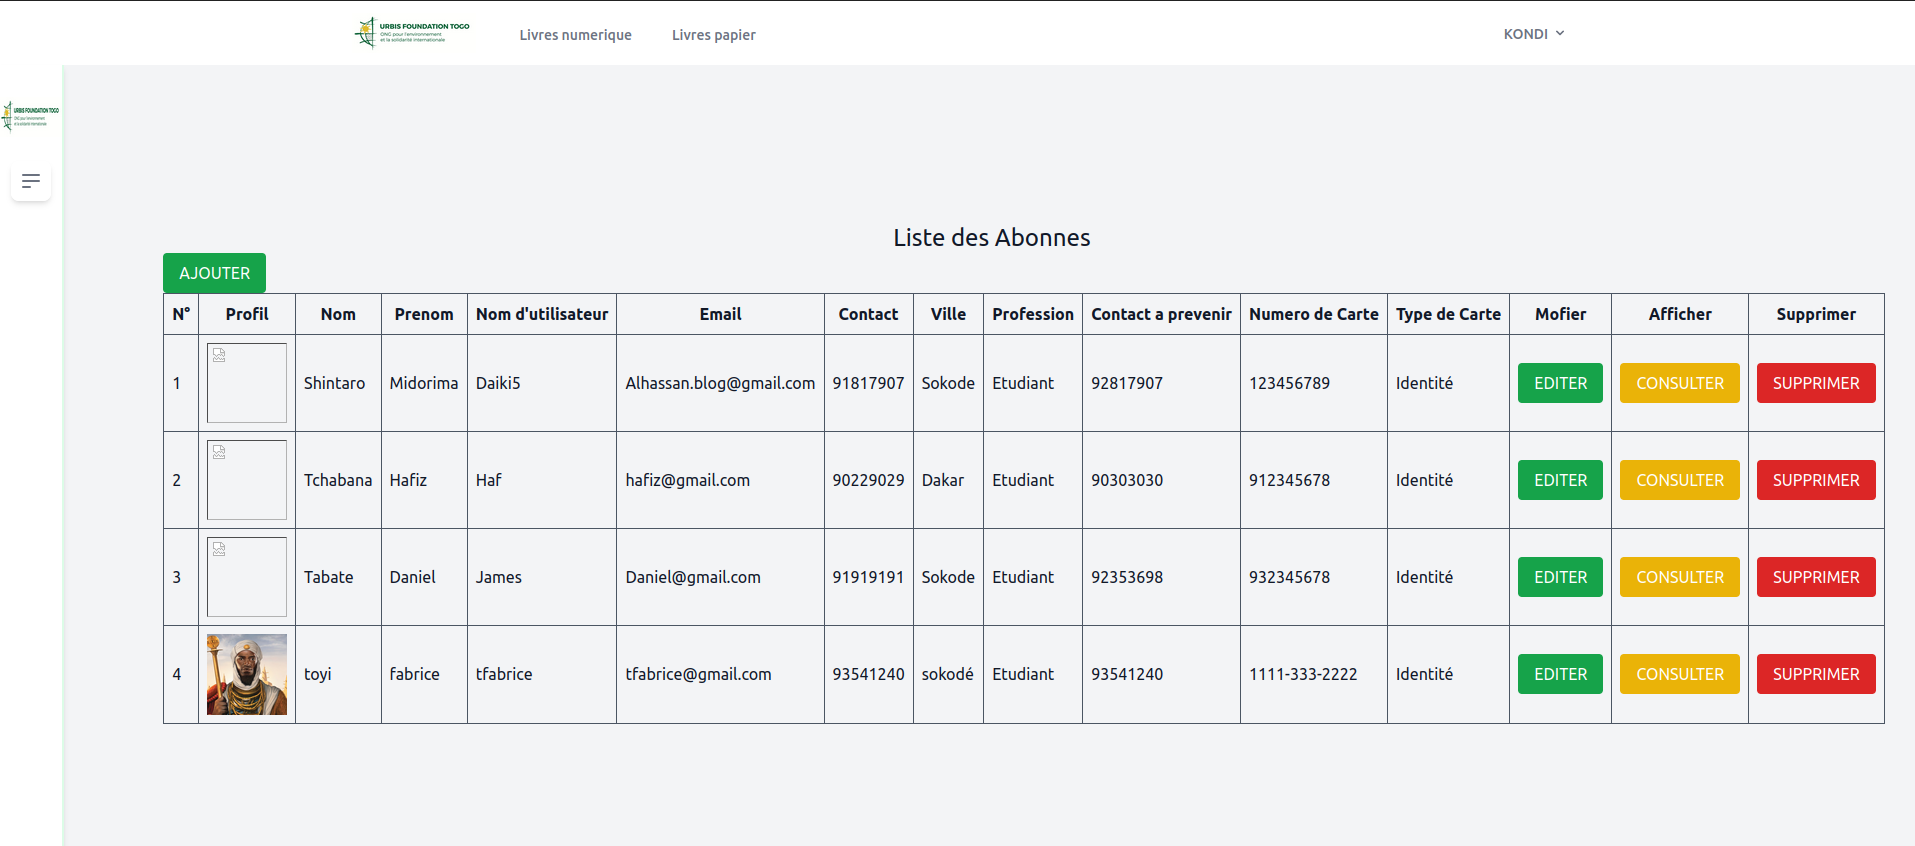
\includegraphics[width=\textwidth]{img/abonnes.png} \\ 
\hline 
\end{tabular} 
\end{center}
Elle contient un bouton \textbf{AJOUTER} et la liste des abonnés afficher dans un tableau.
Pour chaque abonnés vous aurez trois boutons : \textbf{CONSULTER}, \textbf{ÉDITER}, 
\textbf{SUPPRIMER}.\\
\begin{center}
\begin{tabular}{|p{17cm}|}
\hline 
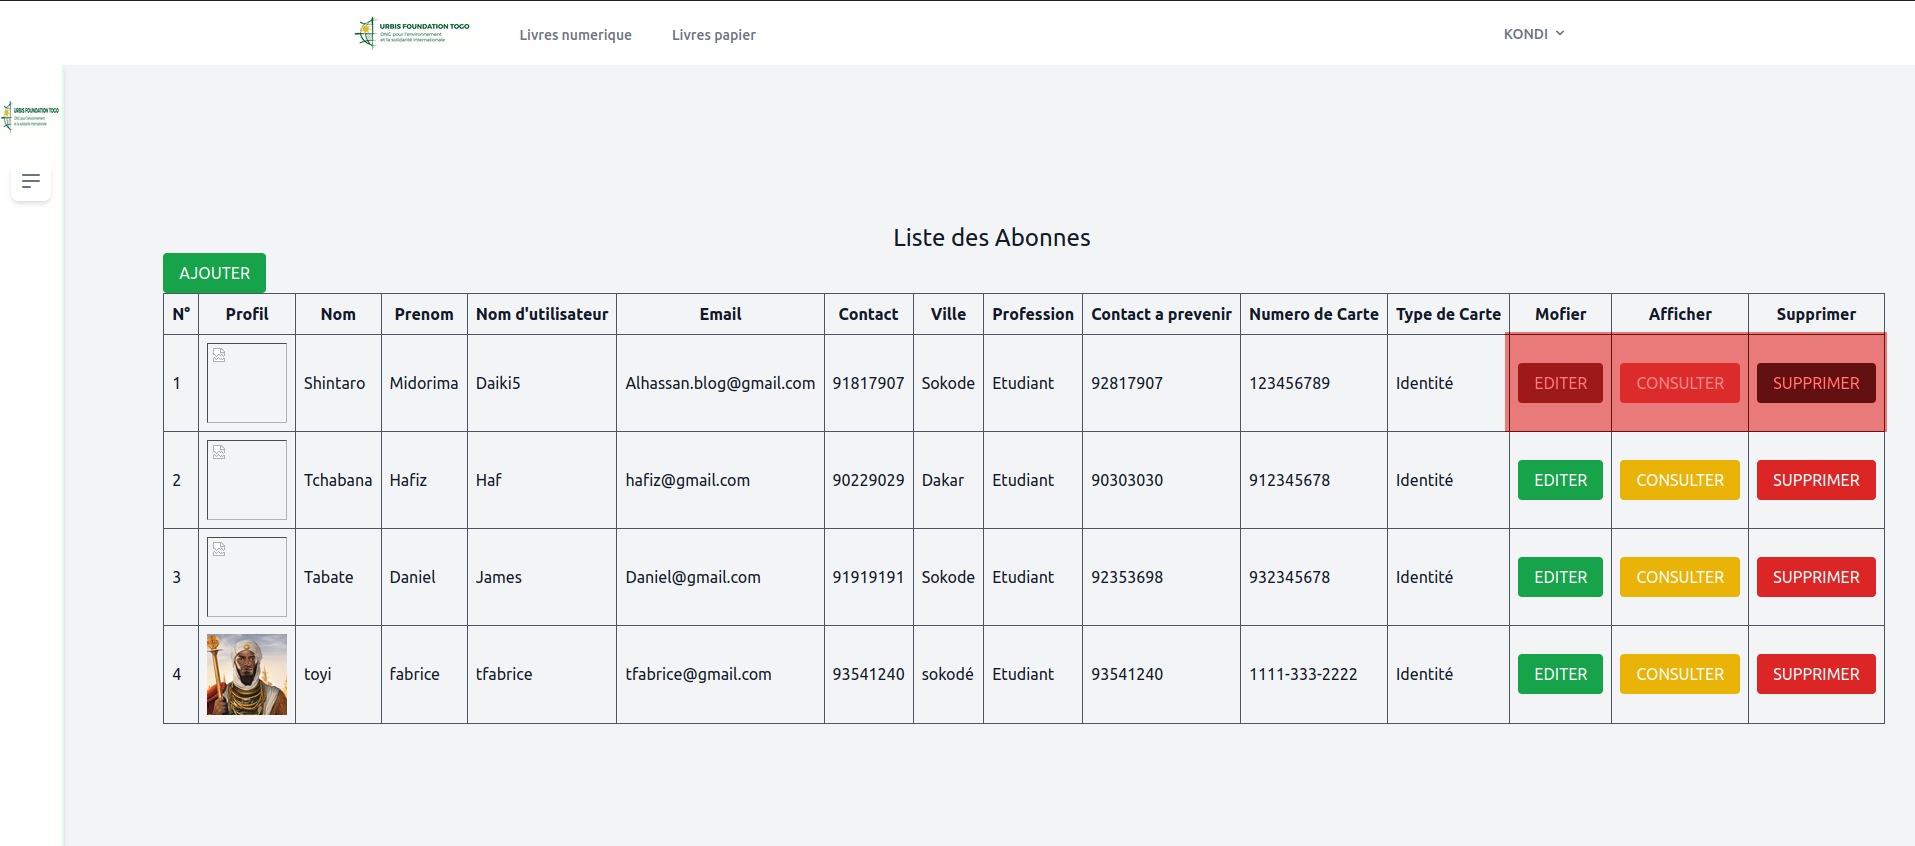
\includegraphics[width=\textwidth]{img/abonnes_btns.png} \\ 
\hline 
\end{tabular} 
\end{center}
\begin{itemize}
\item[•] Bouton \textbf{AJOUTER} : \\
Il permet l'enregistrement d'un nouvelle abonné. Cliquer dessus. C'est fait ? Vous verrez
une nouvelle page apparaître. Elle vous demande de renseigner les informations de l'abonné
puis de cliquer sur le bouton \textbf{ENREGISTRER} pour enregistrer l'abonné.
\begin{center}
\begin{tabular}{|p{17cm}|}
\hline 
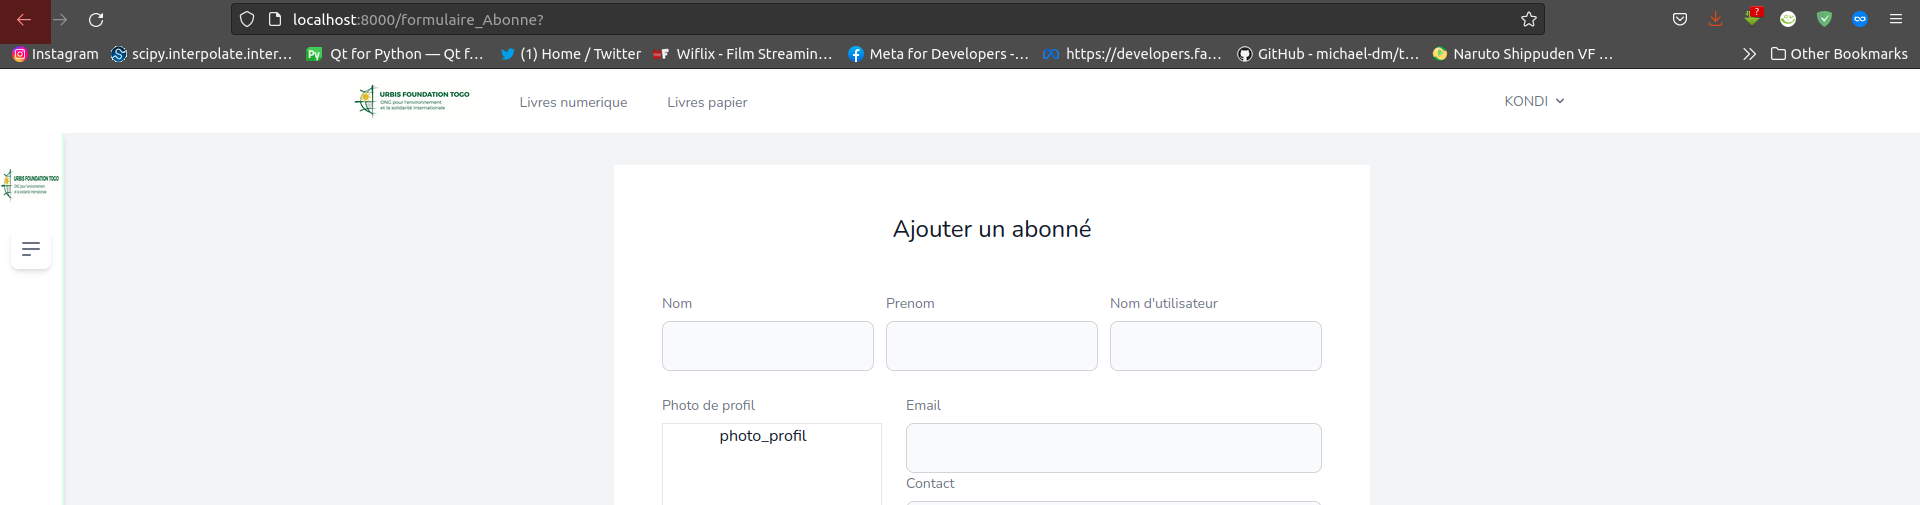
\includegraphics[width=\textwidth]{img/back.png} \\ 
\hline 
\end{tabular} 
\end{center}
ou enregistrer un abonné comme ceci  :\\
\begin{center}
\begin{tabular}{|p{17cm}|}
\hline 
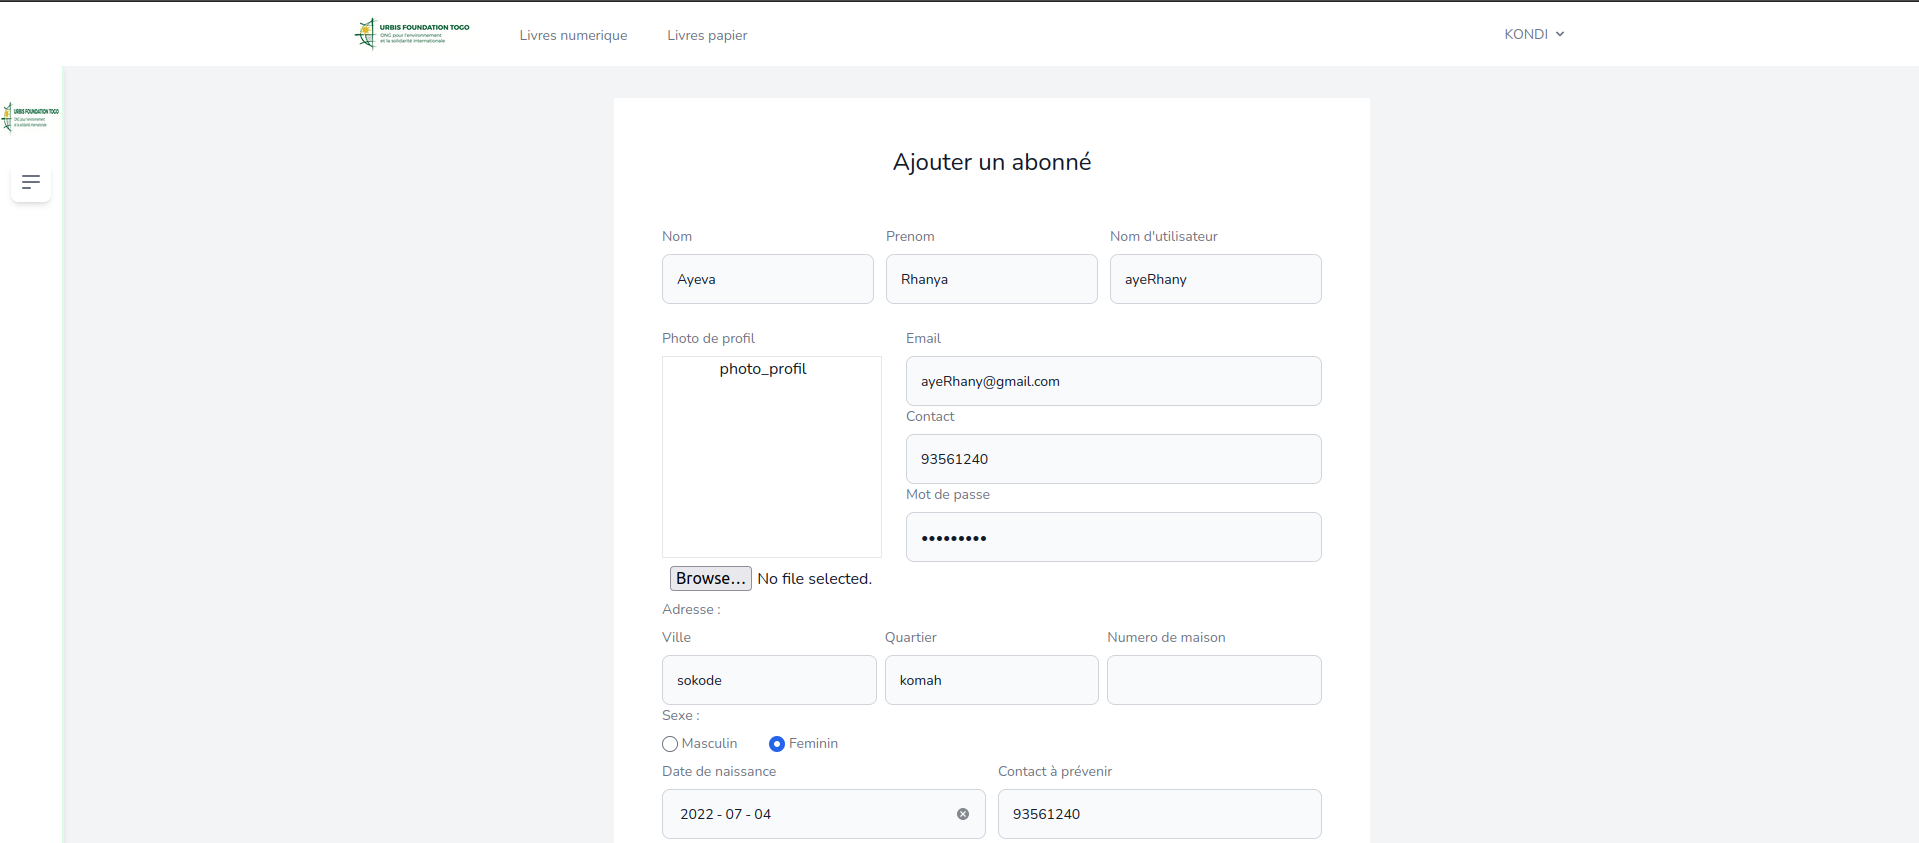
\includegraphics[width=\textwidth]{img/save_abonne.png} \\ 
\hline 
\end{tabular} 
\end{center}
Voici le résultat.\\
\begin{center}
\begin{tabular}{|p{17cm}|}
\hline 
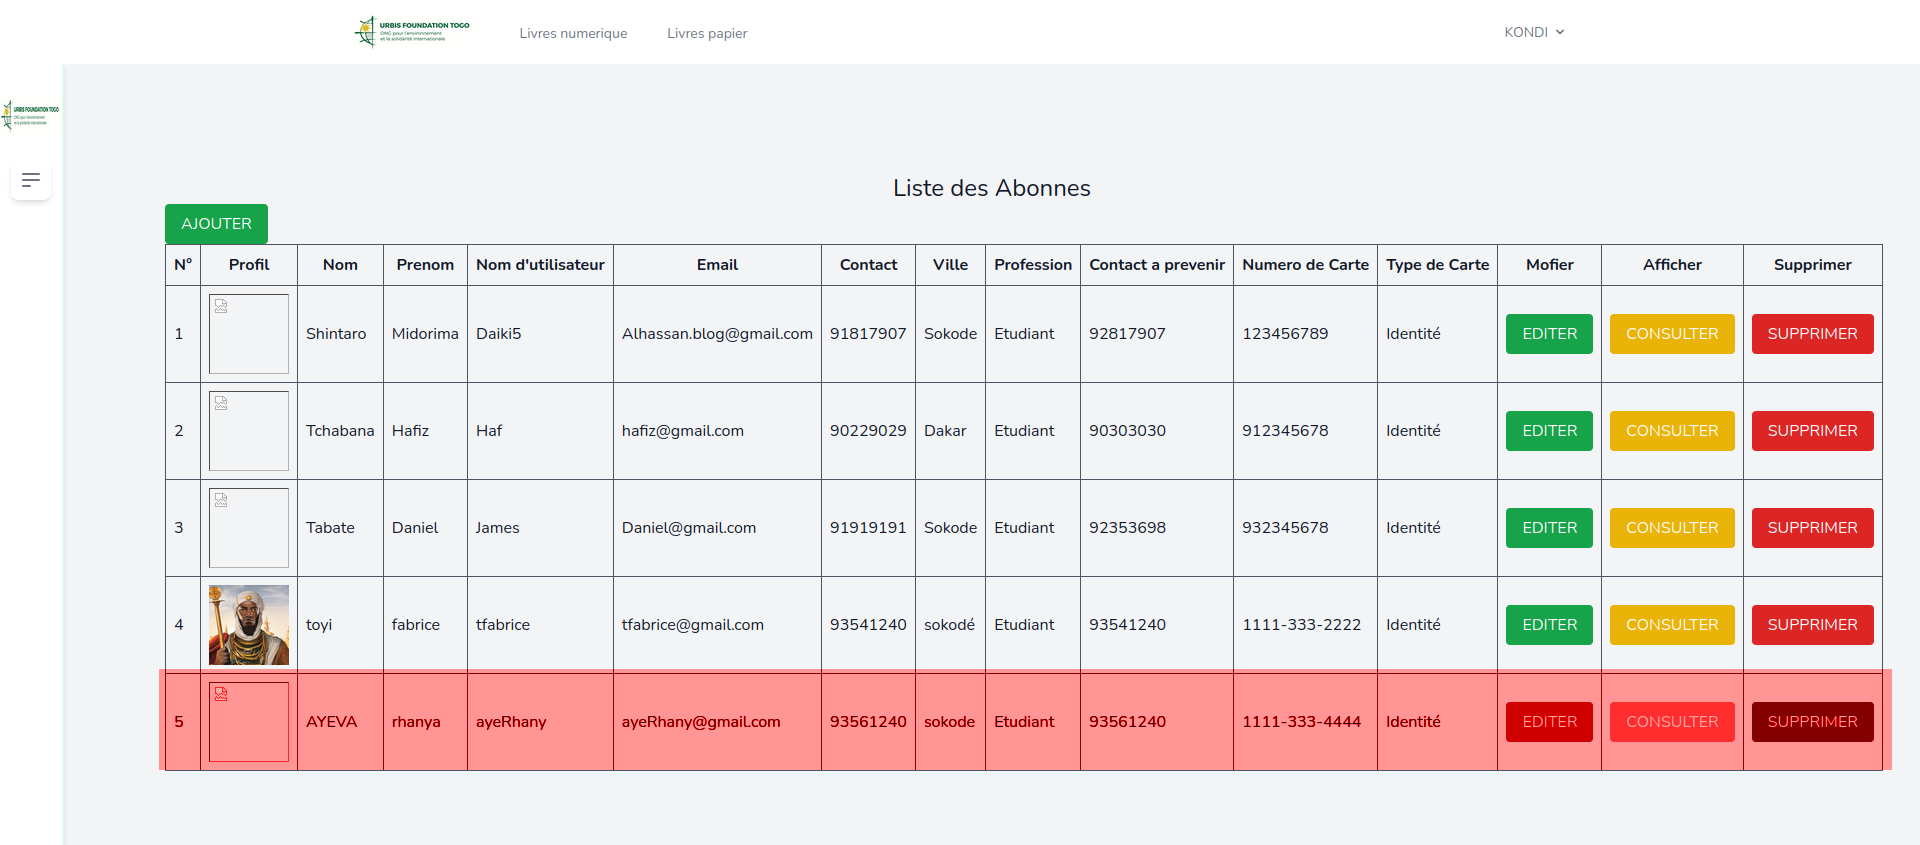
\includegraphics[width=\textwidth]{img/abonnes_2.png} \\ 
\hline 
\end{tabular} 
\end{center}
\textbf{NB:} Tous les champs sont obligatoire pour enregistrer un abonné.
\item[•] Bouton \textbf{EDITER} : \\
Il permet de modifier une ou toute les informations de l'abonné ciblé. Cliquer dessus. Vous verrez s'afficher quelque chose de similaire.
::::::::::::image requise::::::::::::\\
Si nous voulons par exemple changer le numéro de la personne à prévenir pour quelconque 
raison, nous pouvons le ressaisir comme ceci et cliquer sur le bouton modifier.
::::::::::::image requise::::::::::::\\
Voici le résultat.\\
::::::::::::image requise::::::::::::\\
Vous remarquerez que le contact a été modifier.
\item[•] Bouton \textbf{CONSULTER} : \\
Il permet d'accéder à toute les informations de l'abonné ciblé. Cliquer dessus. Vous verrez
s'afficher quelque chose de similaire.
::::::::::::image requise::::::::::::\\
\item[•] Bouton \textbf{SUPPRIMER} : \\
Il permet de supprimer l'abonné ciblé. Cliquer dessus. 
::::::::::::image requise::::::::::::\\
Vous constatez que l'abonné à belle et bien été supprimé.
\end{itemize}
\subsubsection{Sous menu \textbf{Abonnement}}
Ce sous menu permet de garder les traces des payements des abonnés pour leur
abonnement. Après avoir finis d'enregistrer un abonne, vous pouvez enregistrer le 
payement qu'il a effectuer pour l'abonnement (200 FCFA ou 500 FCFA). Pour le faire :
cliquer sur le menu \textbf{Abonnement}. Sélectionner le nom de l'abonné et le tarifs
d'abonnement puis cliquer sur le bouton enregistrer.\\
::::::::::::image requise::::::::::::\\
Cela enregistrera l'opération et vous pouvez voir le résultat. Une fois l'abonnement
enregistrer vous ne pouvez que le consulter, vous ne pouvez pas le supprimer ni même
l'éditer.

\section{Import excel}
Pour enregistrer plusieurs livre papier via une feuille excel, rendez vous sur le
tableau de bord puis sur le menu \textbf{Import excel} choisissez le sous menu 
\textbf{Livre papier}. \\

\begin{center}
\begin{tabular}{|p{17cm}|}
\hline 
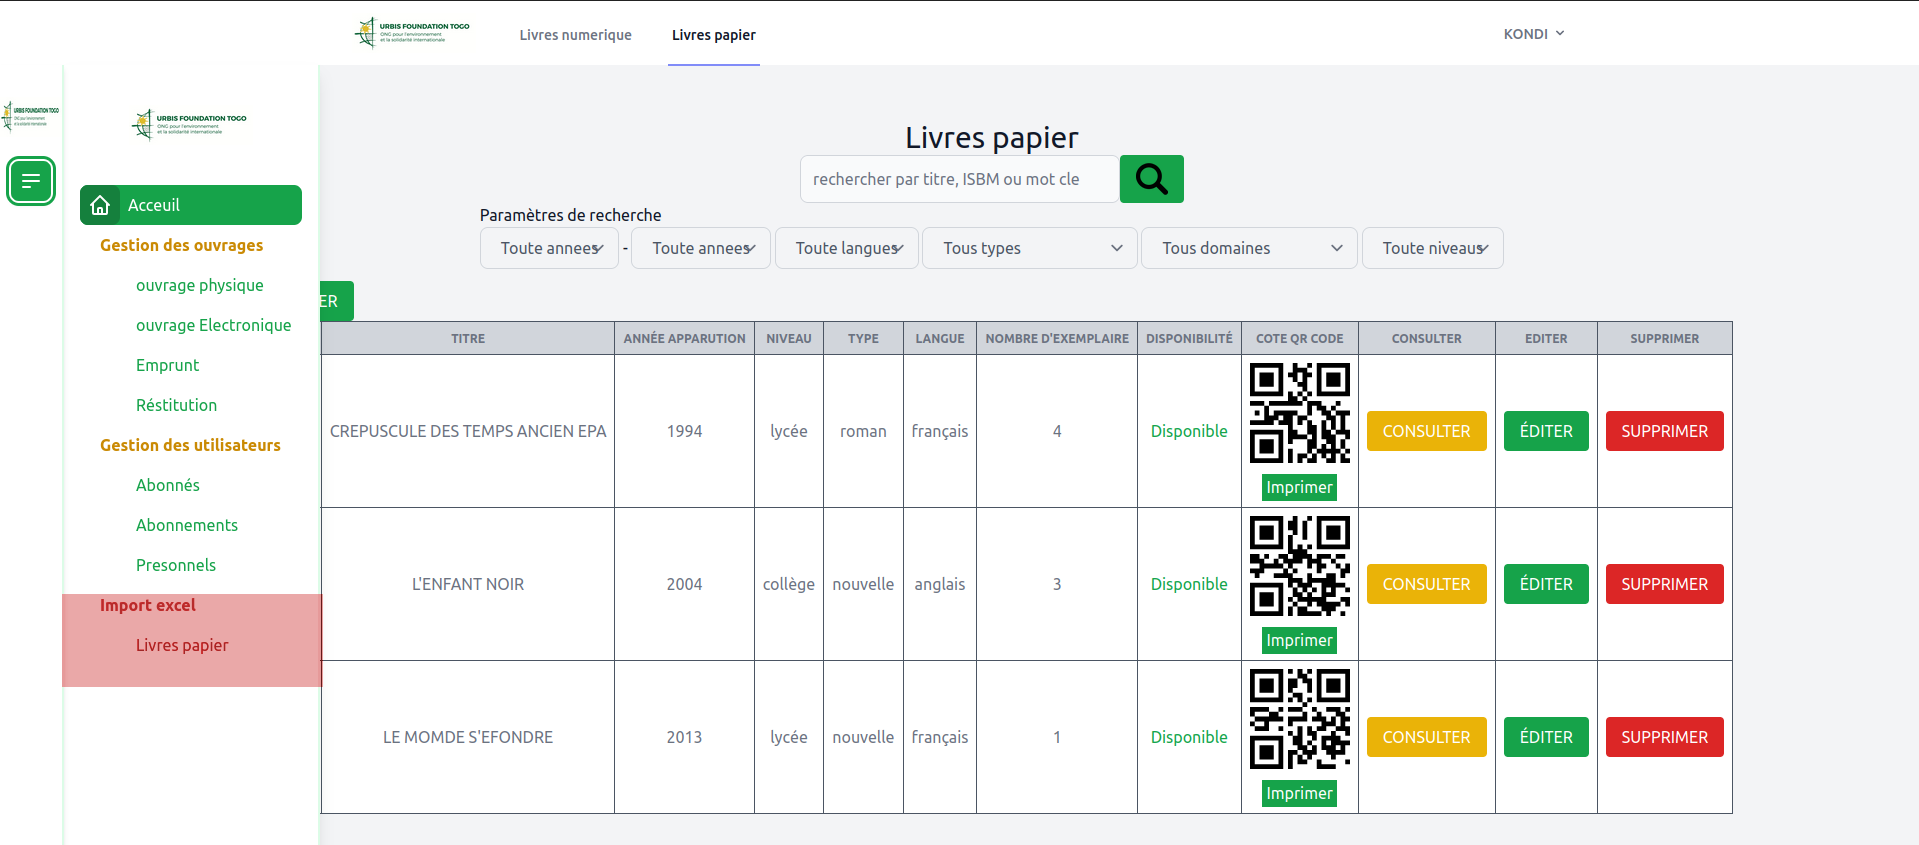
\includegraphics[width=\textwidth]{img/import_excel_menu.png} \\ 
\hline 
\end{tabular} 
\end{center}

Une page s'ouvre. cliquer sur le bouton choisir un fichier,
choisissez votre fichier excel puis appuyez sur le bouton importer.\\
\begin{center}
\begin{tabular}{|p{17cm}|}
\hline 
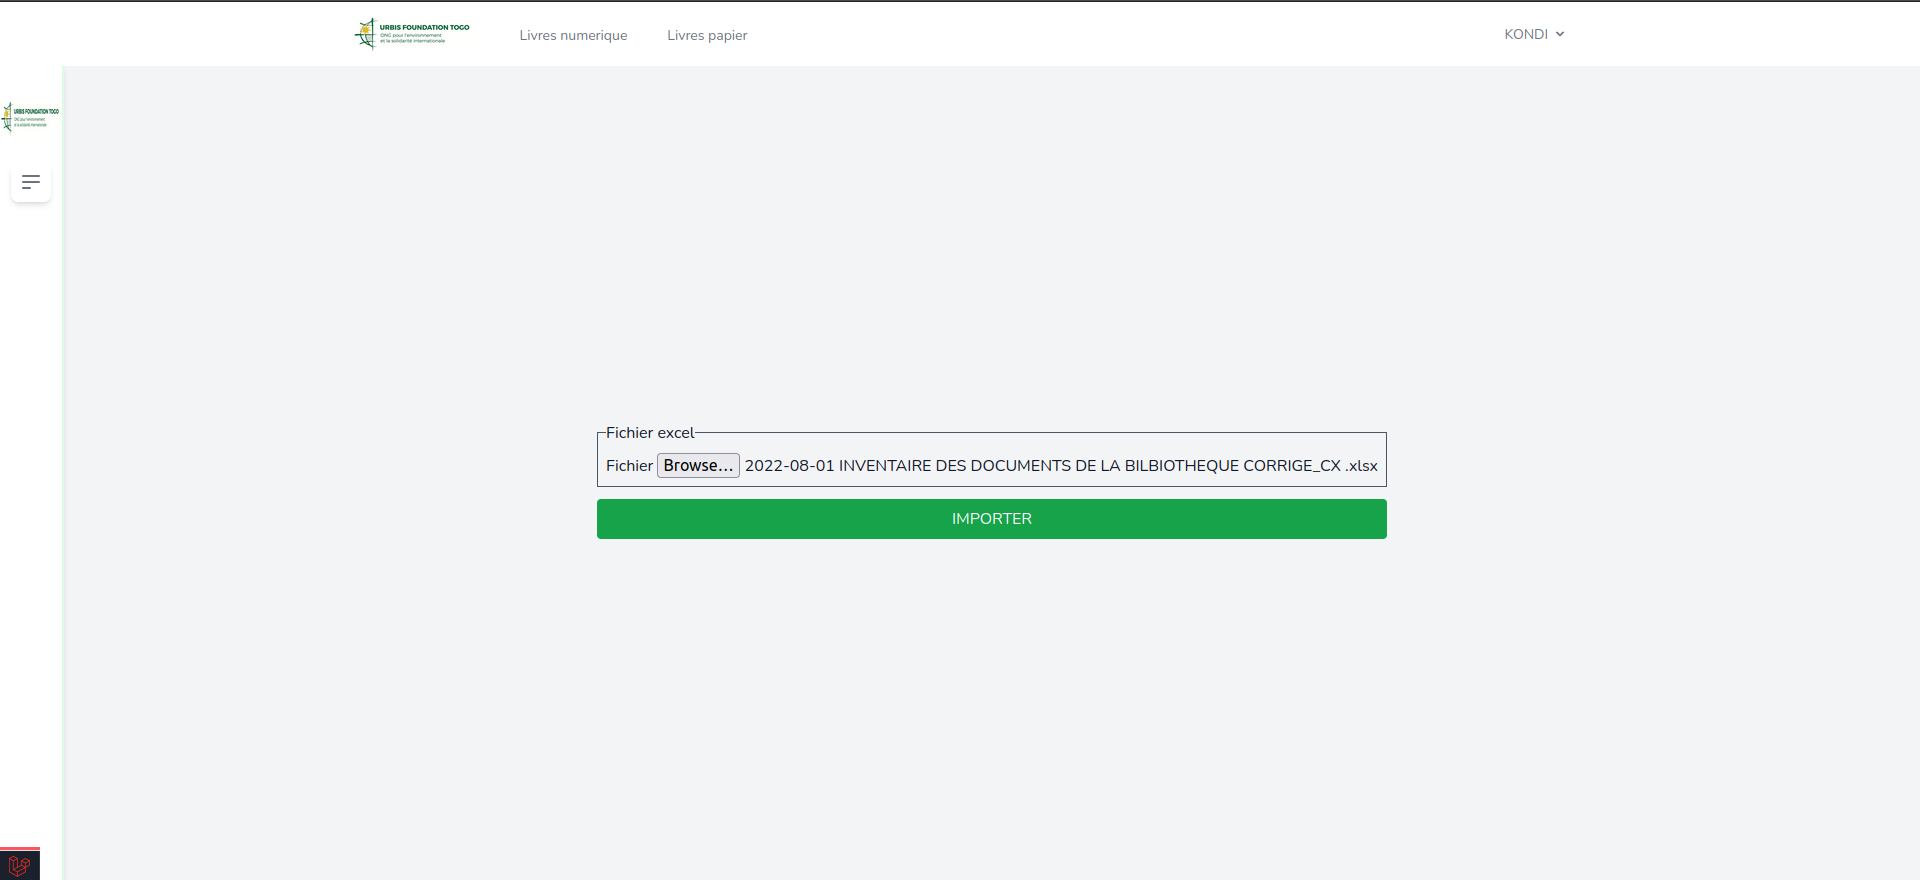
\includegraphics[width=\textwidth]{img/import_excel_content.png} \\ 
\hline 
\end{tabular} 
\end{center}

\textbf{NB:} Le fichier excel ne doit contenir qu'une seul feuille de calcul répondant
aux format çi dessous.\\
\begin{center}
\begin{tabular}{|p{17cm}|}
\hline 
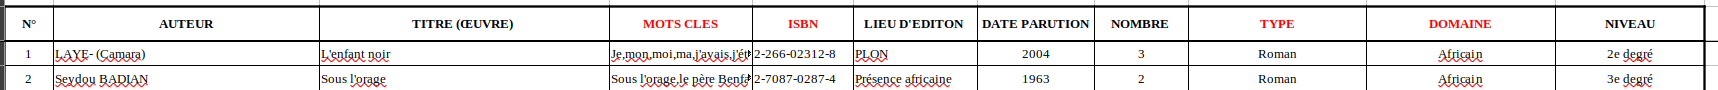
\includegraphics[width=\textwidth]{img/format_excel.png} \\ 
\hline 
\end{tabular} 
\end{center}

\end{document}



